As illustrated in Fig.~\ref{fig:framework}, the proposed framework adopts a dual-branch design that integrates interpretable risk factor detection with predictive modeling in a unified pipeline. Starting from structured clinical data, the framework first applies data inspection and preprocessing procedures, including confirmation of the absence of missing values, standardization where needed, and a separate robustness comparison using winsorization. It then proceeds along two complementary branches: one focuses on identifying clinically relevant variables through multi-angle analysis, while the other performs mortality prediction using multiple machine learning models. The outputs of both branches are subsequently evaluated using standard classification metrics to support patient-level risk assessment.


\begin{figure*}[t]
\centering
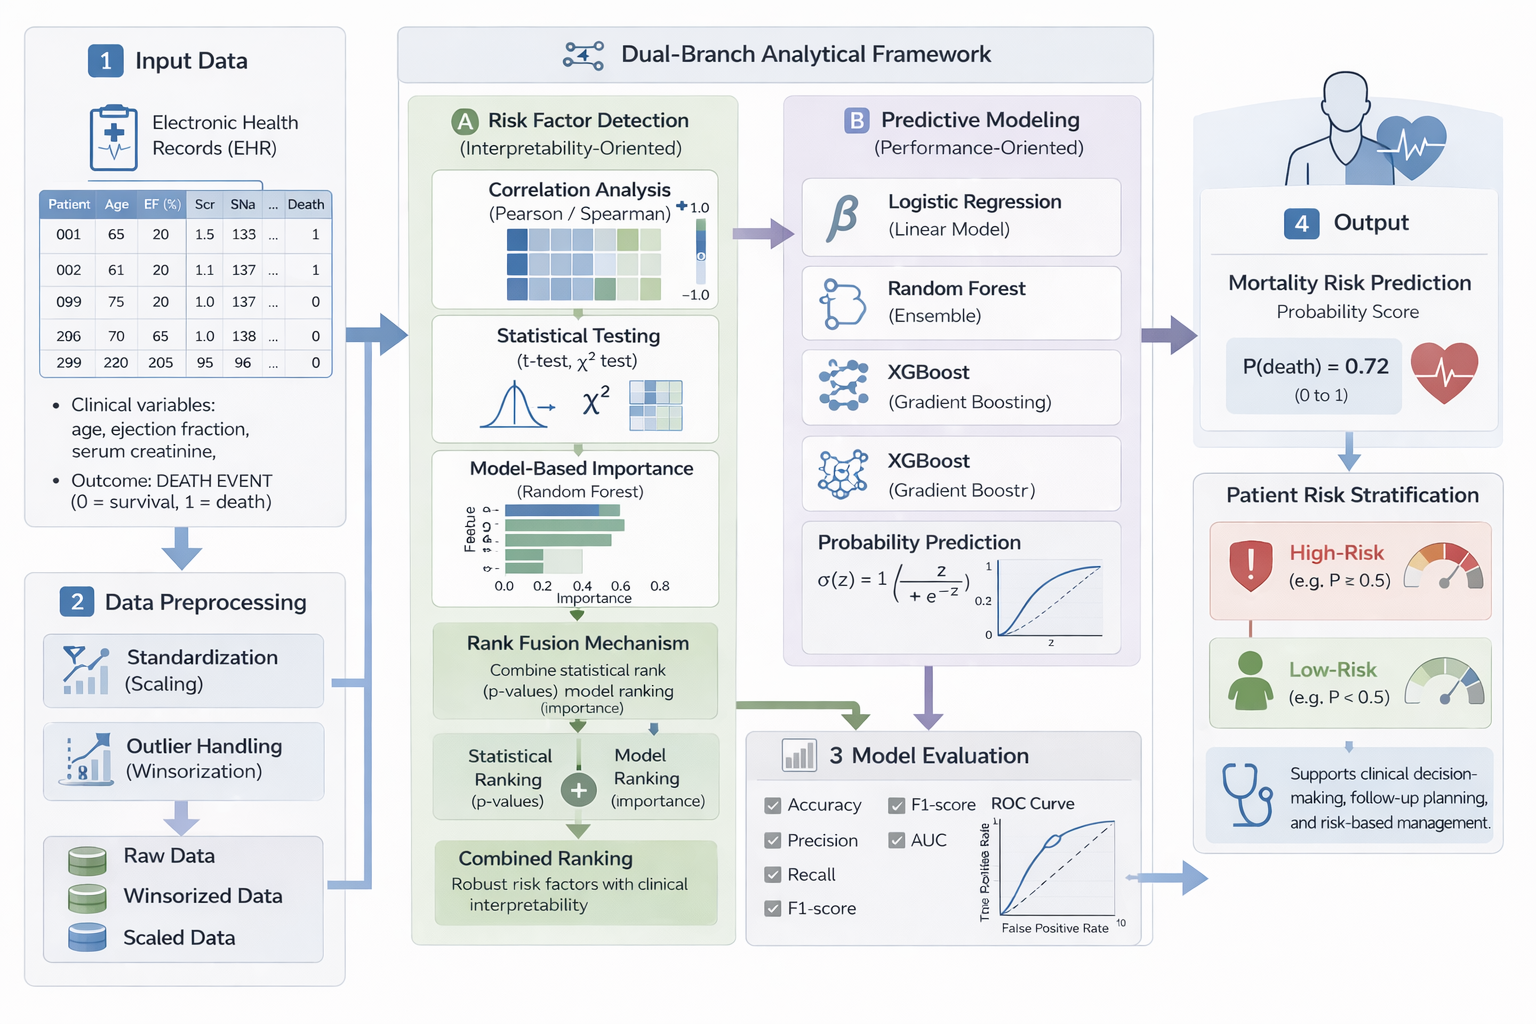
\includegraphics[width=\textwidth]{figures/framework.png}
\caption{
Overview of the proposed dual-branch framework for heart failure mortality prediction, integrating multi-angle risk factor detection with predictive modeling.
}
\label{fig:framework}
\end{figure*}

\subsection{Risk Factor Detection Method}
To identify variables associated with \texttt{DEATH\_EVENT}, a multi-angle analytic framework was used, combining association analysis, correlation structure, and model-based importance. Pairwise correlations among numeric variables were visualized using a correlation heatmap in order to summarize the overall structure of the dataset and highlight potentially related clinical measurements. Univariate outcome comparison was performed using Welch's t-test for continuous variables and chi-square testing for binary variables, providing a statistical screening step for evaluating whether variable distributions differed between patients who survived and those who died during follow-up.

For a continuous variable, the Welch's t-statistic was defined as
\begin{equation}
t = \frac{\bar{x}_1 - \bar{x}_0}{\sqrt{\frac{s_1^2}{n_1} + \frac{s_0^2}{n_0}}},
\end{equation}
where $\bar{x}_1$ and $\bar{x}_0$ denote the group means, $s_1^2$ and $s_0^2$ the group variances, and $n_1$ and $n_0$ the group sample sizes for the death and survival groups, respectively. For binary variables, the chi-square statistic was computed as
\begin{equation}
\chi^2 = \sum_{i}\sum_{j}\frac{(O_{ij} - E_{ij})^2}{E_{ij}},
\end{equation}
where $O_{ij}$ and $E_{ij}$ are the observed and expected cell counts in the contingency table.

Feature importance was estimated using a random forest classifier trained on the full predictor set. Random forest was selected because it can capture nonlinear effects and interactions while providing an interpretable ranking of variable contribution in structured tabular data. Statistical significance and model-based importance were then integrated into a combined ranking procedure. Specifically, each variable received a statistical rank based on ascending p-value from the appropriate univariate test and a model rank based on descending random forest importance. The combined score was defined as:
\begin{equation}
\text{Combined Score}_j = \text{Statistical Rank}_j + \text{RF Rank}_j,
\end{equation}
where a smaller score indicates greater overall prominence. For variables without a valid univariate test ranking, a penalty rank was assigned to avoid overstating their importance. This strategy allowed the study to identify factors that were supported across complementary analytical perspectives rather than by a single criterion alone. Because the \texttt{time} variable reflects follow-up duration and event ascertainment structure, its strong association with mortality was interpreted cautiously and distinguished from baseline biological risk factors.

\subsection{Predictive Modeling Method}
Mortality prediction was evaluated using four supervised learning models: logistic regression (LR), random forest (RF), extreme gradient boosting (XGBoost), and multilayer perceptron (MLP). Logistic regression was included as a conventional and interpretable baseline for binary classification. For patient feature vector $\mathbf{x}$, logistic regression estimates the probability of death as
\begin{equation}
P(y=1 \mid \mathbf{x}) = \sigma(\beta_0 + \boldsymbol{\beta}^{\top}\mathbf{x}) = \frac{1}{1 + e^{-(\beta_0 + \boldsymbol{\beta}^{\top}\mathbf{x})}}.
\end{equation}

Random forest was used as a tree-based ensemble method that aggregates predictions from multiple decision trees and is well suited to tabular clinical data with nonlinear relationships. The final prediction probability can be expressed as the average output across $B$ trees:
\begin{equation}
\hat{P}_{RF}(y=1 \mid \mathbf{x}) = \frac{1}{B}\sum_{b=1}^{B} T_b(\mathbf{x}),
\end{equation}
where $T_b(\mathbf{x})$ denotes the probability estimate from the $b$th tree.

XGBoost was included as a gradient boosting method that builds an additive ensemble of weak learners in a stage-wise manner. Its prediction function can be written as
\begin{equation}
\hat{y}_i = \sum_{k=1}^{K} f_k(\mathbf{x}_i), \qquad f_k \in \mathcal{F},
\end{equation}
where each $f_k$ is a regression tree and $\mathcal{F}$ denotes the space of allowable trees. This framework is effective for learning nonlinear decision boundaries while controlling model complexity through regularization.

The MLP model was used as a simple neural-network baseline. For one hidden layer, the mapping can be expressed as
\begin{equation}
\hat{y} = \sigma\left(\mathbf{W}_2 \, g(\mathbf{W}_1 \mathbf{x} + \mathbf{b}_1) + \mathbf{b}_2\right),
\end{equation}
where $\mathbf{W}_1$ and $\mathbf{W}_2$ are weight matrices, $\mathbf{b}_1$ and $\mathbf{b}_2$ are bias terms, $g(\cdot)$ is the hidden-layer activation function, and $\sigma(\cdot)$ is the output sigmoid function. The MLP was included to assess whether a modest neural architecture provided any advantage over classical machine learning models in this small-sample setting.
